\documentclass{article}
\usepackage{amsmath}
\usepackage{amssymb}
\usepackage{graphicx}
\usepackage{hyperref}
\usepackage[version=4]{mhchem}

\title{Problem 14}
\date{}

\begin{document}
\maketitle

\section*{Problem}
(AMC) In the adjoining figure \(T P\) and \(T^{\prime} Q\) are parallel tangents to a circle of radius \(r\), with \(T\) and \(T^{\prime}\) the points of tangency. \(P T^{\prime \prime} Q\) is a third tangent with \(T^{\prime \prime}\) as point of tangency. If \(T P=4\) and \(T^{\prime} Q=9\) then \(r\) is\\
(A) \(25 / 6\) (B) 6 (C) 25/4\\
(D) a number other than \(25 / 6,6,25 / 4\)\\
(E) not determinable from the given information\\
\centering
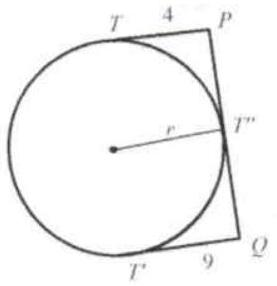
\includegraphics[width=\textwidth]{images/156(2).jpg}

\section*{Solution}
(B).\\
\(r=\sqrt{T P \times T^{\prime} Q}=\sqrt{4 \times 9}=6\)\\
\centering

\includegraphics[width=\textwidth]{images/161.jpg}


2. Draw the line segments connecting special points on the circumference
2.1. \(A B\) is the diameter. Connect \(A C\) and \(B C\). We have \(\angle C=90^{\circ}\).\\
\centering
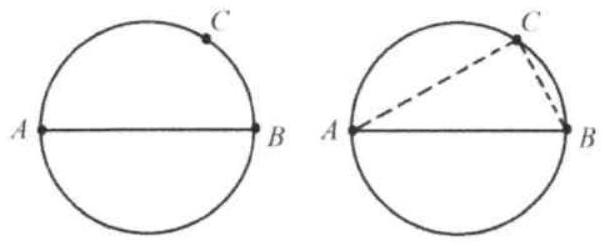
\includegraphics[width=\textwidth]{images/162(1).jpg}

Theorem 6.7a. An angle inscribed in a semicircle is a right angle.

Theorem 6.7b. The measure of an inscribed angle equals one-half the measure of its intercepted arc. \(\angle C=\frac{180^{\circ}}{2}=90^{\circ}\)\\
\centering

\includegraphics[width=\textwidth]{images/162.jpg}\\
2.2. \(A B C\) is a triangle. \(D\) is a point on the circumference. Connect \(D B, D A\). We have \(\angle B A C=\angle B D C=\alpha ; \angle D A C=\angle D B C=\beta ; \angle A D B=\angle A C B=\gamma\), \(\angle A C D=\angle A B D=\theta\).\\
\centering
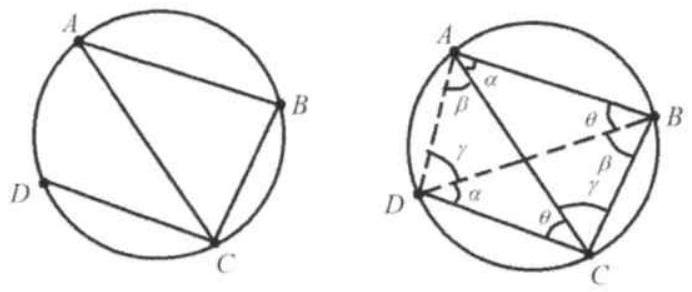
\includegraphics[width=\textwidth]{images/162(2).jpg}

Theorem 6.8. In the same or congruent circles, congruent inscribed angles have congruent intercepted arcs.

\end{document}
